\documentclass[12pt,letterpaper]{article}
\usepackage{./preamble}
\usepackage{amsmath}

%%%%%%%%%%%%%%%%%%%%%%%%%%%%%%%%%%%%%%%%%%
%%%% Edit These for yourself
%%%%%%%%%%%%%%%%%%%%%%%%%%%%%%%%%%%%%%%%%%
\newcommand\course{Computational Statistics}
\newcommand\hwnumber{3}
\newcommand\userID{Davi Sales Barreira}
\DeclareRobustCommand{\rchi}{{\mathpalette\irchi\relax}}
\newcommand{\irchi}[2]{\raisebox{\depth}{$#1\chi$}}
\newcommand*{\QEDA}{\hfill\ensuremath{\blacksquare}}%

\begin{document}
% \textbf{\Large Worksheet completed with Octave.}

\section*{Exercise 1 (Gibbs Sampler)}
\begin{enumerate}[leftmargin=!,labelindent=5pt]
\item First, let $X' = X^{(t)}$, $X = X^{(t-1)}$, $Y' = Y^{(t)}$ and
$Y = Y^{(t-1)}$
. Then:
$$
K^S((x,y),(x',y')) = \pi_{Y\mid X}(y' \mid x) \pi_{X \mid Y}(x' \mid y')
$$

Then, to show that it is not reversible:
$$
\pi(x,y)K((x,y),(x',y')) = \pi(x,y) \pi(y' \mid x) \pi(x' \mid y')
$$
$$ 
\pi(x',y')K((x',y'),(x,y)) = \pi(x',y') \pi(y \mid x') \pi(x \mid y)
$$
$$
\therefore
$$
$$
\frac{\pi(x,y)K((x,y),(x',y'))}
{\pi(x',y')K((x',y'),(x,y))} =
\frac{\pi(x,y) \pi(y' \mid x) \pi(x' \mid y')}
{\pi(x',y') \pi(y \mid x') \pi(x \mid y)} = 
\frac{\pi(y)\pi(y' \mid x)}
{\pi(y')\pi(y \mid x')} \neq 1
$$
Therefore, it is not reversible.
\qed

\item First, the kernel expression:
$$
K(x, x') = \int \pi(y' \mid x) \pi(x' \mid y') dy'
$$

Now, let's show that it is $\pi_X$-reversible.
$$
\pi(x')K(x', x) = \pi(x') \int \pi(y \mid x') \pi(x \mid y) dy
=
\int \pi(x') \frac{\pi(y,x')}{\pi(x')}\pi(x\mid y) dy =
$$
$$
=
\int \pi(y,x') \pi(x \mid y) dy = 
\int \pi(y,x') \frac{\pi(x,y)}{\pi(y)}dy =
\int \pi(x,y) \frac{\pi(x',y)}{\pi(y)}dy =
$$
$$
= \pi(x)\int \pi(y \mid x) \pi(x' \mid y)  dy = \pi(x)K(x,x')
$$
\qed

\item First, the kernel expression is:
$$
K^R((x,y),(x',y')) = 
\pi(y' \mid x)\pi(x' \mid y')0.5 + \pi(x' \mid y)\pi(y' \mid x')0.5
$$
Note that it is half the density of sampling first from $y$ plus 
half the density of sampling first from $x$.

Now, let's show that it is reversible:
$$
\frac{\pi(x,y)[\pi(y' \mid x)\pi(x' \mid y')0.5 +
\pi(x' \mid y)\pi(y' \mid x')0.5]}
{
\pi(x',y')[\pi(y \mid x')\pi(x \mid y')0.5 +
\pi(x \mid y')\pi(y \mid x)0.5 ]
} = 
$$
$$ =
\frac{
	\frac{\pi(y' \mid x)}
	{\pi(y')}
	+
	\frac{\pi(x' \mid y)}
	{\pi(x')}
}
{
	\frac{\pi(y \mid x')}
	{\pi(y)}
	+
	\frac{\pi(x \mid y')}
	{\pi(x)}
} = 
1
$$
\qed
\end{enumerate}

\newpage
\section*{Exercise 2 (Metropolis-within-Gibbs)}
\begin{enumerate}[leftmargin=!,labelindent=5pt]
\item Note that:
$$
\alpha(X_1 \mid X_1^{(t-1)}, X_2^{(t-2)}) =
min \left\{
1,
\frac{\pi(X_1' , X_2^{(t-1)})\pi(X_1^{(t-1)}\mid X_2^{(t-1)})}
{\pi(X_1^{(t-1)} , X_2^{(t-1)})\pi(X_1'\mid X_2^{(t-1)})}
\right\} = min \{1, 1\}
$$
Therefore, we get a systematic scan Gibbs sampler, where one
samples $X^t_1 \sim \pi(\cdot \mid X_2^{(t-1)})$, then we accept,
since $\alpha=1$, and finally sample $X_2^t \sim
\pi(\cdot \mid X_1^{(t)})$.
\qed

\item First, let's write the kernel. Since we only accept or reject
the variabel $X_1$, the kernel is the M-H kernel multiplied by the
probability density function of $\pi_{X_2\mid X_1}(X_2\mid X_1)$. Let
$X_1^t, X_2^t = Y_1, Y_2$:
$$
K((x_1,x_2),(y_1, y_2)) =
(q(y_1 \mid x_1, x_2)\alpha(y_1 \mid x_1,x_2)) +
(1 - a(y_1 \mid x_1, x_2))\delta_{y_1}(x_1)\pi_{(Y_2\mid Y_1}(y_2 \mid y_1)
$$
Note that $\alpha = 1$. With that, we show that the kernel is invarant:

$$
\int \int
K((x_1,x_2),(y_1, y_2))\pi(x_1,x_2) dx_1 dx_2 =
\int \int \pi(y_1 \mid x_2)\pi(y_2 \mid y_1) \pi(x_1, x_2)dx_1 dx_2 =
$$
$$=
\int \pi(y_1 \mid x_2) \pi(y_2 \mid y_1) \pi(x_2) dx_2 =
\int \pi(y_1, x_2)\pi(y_2 \mid y_1) dx_2 = \pi(y_1, y_2)
$$
\qed

\end{enumerate}

\newpage
\section*{Exercise 3 (Metropolis-Hastings and Gibbs Sampler)}
\begin{enumerate}[leftmargin=!,labelindent=5pt]
\item  Let's show that the chain is reversible. If $x=y$, it is trivially
reversible. If $x \neq y$, then:
$$
T(x,y) \pi(x) = \alpha(x,y)q(x,y)\pi(x) =
\frac{\gamma(x,y)}{\pi(x)q(x,y)}q(x,y)\pi(x) = \gamma(y,x) =
$$
$$
= \alpha(y,x) q(y,x) \pi(y) = T(y,x) \pi(y)
$$
\qed

\item First, let's verify that it is the M-H algorithm:
$$
\alpha = \frac{\gamma(x,y)}{\pi(x)q(x,y)} = 
\frac{min \{  \pi(x) q(x,y), \pi(y) q(y,x) \}}
{\pi(x) q(x,y)} =
min \left \{
	1, \frac{\pi(y)q(y,x)}
	{\pi(x)q(x,y)}
\right\}
$$

Now, let's give the Barker acceptance ratio:
$$
\alpha(x,y) = \frac{\pi(x)q(x,y)\pi(y)q(y,x)}
{\pi(x)q(x,y)+\pi(y)q(y,x)} =
\frac{\pi(y)q(y,x)}{\pi(x)q(x,y) + \pi(y)q(y,x)}
$$
\qed

\item Let's consider $x \neq y$. Note that:
$$
\frac{1}{\pi(x)q(x,y)}
\geq
\frac{1}{\pi(x)q(x,y) + \pi(y)q(y,x)}
$$
$$
\therefore
$$
$$
\frac{\pi(y)q(y,x)q(x,y)}{\pi(x)q(x,y)}
\geq
\frac{q(x,y)\pi(y)q(y,x)}{\pi(x)q(x,y) + \pi(y)q(y,x)}
$$

Finally, if $\frac{\pi(y)q(y,x)q(x,y)}{\pi(x)q(x,y)} \leq 1$, then:

$$
min\left \{
1,
\frac{\pi(y)q(y,x)q(x,y)}{\pi(x)q(x,y)}
\right\}
\geq
\frac{q(x,y)\pi(y)q(y,x)}{\pi(x)q(x,y) + \pi(y)q(y,x)}
$$

We conclude that the M-H algorithm provides estimators with
lower asymptotic variance than Barker's algorithm.

\item First, since the probability of chosing and index is the same
for both algorithms, it is not important when showing which
kernel is bigger of equal than the other. Now, consider $x \neq y$.

Modified: $T(x_k^{(t-1)}, x_k^*) =
min\left\{
1, \frac{1- \pi(x_k^{(t-1)} \mid x_{-k})}{1 -  \pi(x_k^* \mid x_{-k})}
\right\}
\frac{\pi(x_k^* \mid x_{-k})}{1- \pi(x_k^{(t-1)} \mid x_{-k})}$

Standard: $T(x_k^{(t-1)}, x_k^*) = \pi(x_k^* \mid x_{-k})$

Let's consider both cases for the Modified kernel, hence, when
$\alpha = 1$ and
$\alpha =
\frac{1- \pi(x_k^{(t-1)} \mid x_{-k})}{1 -  \pi(x_k^* \mid x_{-k})} $
First, since $1- \pi(x_k^{(t-1)} \mid x_{-k})\leq 1$, we have:
$$
1 \cdot\frac{\pi(x_k^* \mid x_{-k})}{1- \pi(x_k^{(t-1)} \mid x_{-k})}
\geq
\pi(x_k^* \mid x_{-k})
$$

Also:
$$
\frac{1- \pi(x_k^{(t-1)} \mid x_{-k})}{1 -  \pi(x_k^* \mid x_{-k})}
\cdot\frac{\pi(x_k^* \mid x_{-k})}{1- \pi(x_k^{(t-1)} \mid x_{-k})}
\geq
\pi(x_k^* \mid x_{-k})
$$
Therefore, the modified kernel provides estimators
with lower assymptotic variance.
\qed
\end{enumerate}

\newpage
\section*{Exercise 4 (Metropolis-Hastings)}
\begin{enumerate}[leftmargin=!,labelindent=5pt]
\item Let $Y = X'$, $\theta = v'$:
$$q(y \mid x) = \int f(v \mid x) g(y \mid v) dv$$
$$
\alpha_{MH} = min \left \{ 1,
\frac{\pi(y)\int f(v \mid y) g(x \mid v) dv}
{\pi(x)\int f(v \mid x) g(y \mid v) dv}
\right \}
$$
Since we the density function $f(v \mid x)$ is unknown, then we cannot 
evaluate this $\alpha_{MH}$.

\item Let's show that the chain is invariant:
$$
\int \int \pi(x,v) g(y \mid v) f(\theta \mid y)
\cdot min \left \{
1, \frac{\pi(y)g(x \mid \theta)}{\pi(x)g(y\mid v)}
\right\} dv dx = 
$$
If $\alpha =1 $, then

$$
\int \pi(v) g(y \mid v) f(\theta \mid y)
\cdot 1
dv = f(\theta \mid y) \pi(y) = \bar\pi(y, \theta)
$$

Else:
$$
\int \int \pi(x,v) g(y \mid v) f(\theta \mid y)
\cdot 
\frac{\pi(y)g(x \mid \theta)}{\pi(x)g(y\mid v)}
dv dx = 
\int \pi(y) f(\theta \mid y) g(x \mid \theta) dx =
$$
$$
= \pi(y) f(\theta \mid y) = \bar\pi(y, \theta)
$$

Finally, $\bar\pi(y) = \int \bar\pi(y,\theta) d\theta = 
\int \pi(y) f(\theta \mid y) d\theta = \pi(y)$.

\qed

\item First, note that $min(U,V) = \frac{U+V -\mid U - V \mid}{2}$, hence:
$$
E \left[
	\frac{U + V - \mid U - V \mid}{2}
\right] = 
\frac{E[U] + E[V] - E[\mid U - V \mid] }{2}
$$
Without loss of generality, assume $E[U] \geq E[V]$. Then:
$$
E[\mid U - V \mid] \geq E[U] - E[V]
$$
$$
\therefore
$$
$$
\frac{E[U] + E[V] - E[\mid U - V \mid] }{2} \leq
\frac{E[U] + E[V] - E[U]- E[V]}{2} = E[V]
$$
\qed

\item Couldn't solve.
\end{enumerate}

\newpage
\section*{Exercise 5 (Thinning of a Markov chain)}
\begin{enumerate}[leftmargin=!,labelindent=5pt]
\item
$$
E[y^2] + \alpha^2E[Z^2] + 2\alpha |E[YZ]| \geq 0
$$
Therefore, we have a second degree polynomial in $\alpha$ that is
greater or equal than 0. Hence, we know that $b^2 - 4ac \leq 0$, which
means:
$$
(2 E[YZ])^2 - 4E[Z^2]E[Y^2] \leq 0 \therefore
E[Z^2]E[Y^2] \geq |E[YZ]|
$$
\qed

\item Using the inequality from the previouse question, we have:
$$
Cov(Y,Z) = E[(Y-E[Y])(Z - E[Z])] \therefore
Cov(Y,Z)^2 \leq E[(Y-E[Y])^2]E[(Z - E[Z])^2]
$$
$$
\therefore
$$
$$
\sqrt{Var(Y)Var(Z)} \geq Cov(Y,Z)
$$
Since $Var(Y) = Var(Z)$ by hypothesis, then:

$$
Var(Y) \geq Cov(Z,Y)
$$
\qed

\item Couldn't prove the inequality. But, given that it is true,
it implies that thinning doesn't improve the results, in other words,
it doesn't lower the variance.
\end{enumerate}

\newpage
\section*{Simulation question (Probit model - Gibbs and M-H)}
\begin{enumerate}[leftmargin=!,labelindent=5pt]
\item 
In the probit model we have the similar situation that we have for the linear regression,
hence:
$$
Y = \beta_0 + \beta_1 x_1 + ... + \beta_n x_n
$$
But $Y = 0$ or $1$, so we have to transform the linear equation to fall between 0 and 1.
To do that, we use the cdf for the normal distribution.
$$
Y = \phi(\beta_0 + \beta_1 x_1 + ... + \beta_n x_n)
$$
Note that the cdf will guarantee a value between 0 and 1.
Thus, we can generate synthetic dataset $Y$ by choosing values
for a $beta$ than sampling $X$ from a multivariate normal with
chosen parameters, and finally,
applying the probit formulat to get $Y$. For this simulation,
we set 
$$
\beta =
\begin{bmatrix}
1 \\ -1
\end{bmatrix}
, X \sim MVN \left ( \mu = 
\begin{bmatrix}
0 \\ 0
\end{bmatrix}
, \Sigma = 
\begin{bmatrix}
1 & 0 \\ 0 & 2
\end{bmatrix}
\right)
$$

\begin{figure}[H]
    \centering
    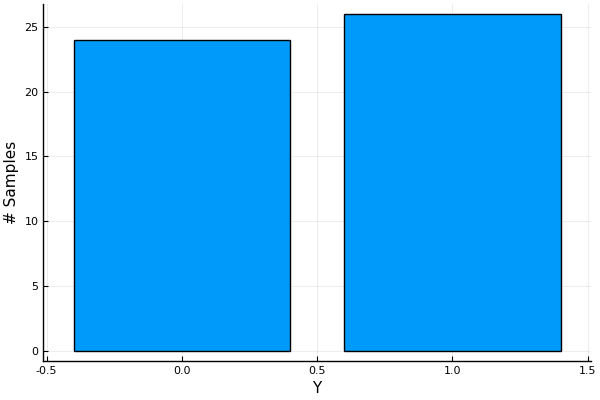
\includegraphics[width=10cm]{images/Ex6_1.png}
    \caption{Synthetic dataset Y of size 50.
    $\beta = [1, -1], X \sim MVN(
    \mu, \Sigma)$.
    }
    \label{fig:1}
\end{figure}

\item 

$$\pi(\beta) = N (0, B)$$

For a $p \times p$ covariance matrix B, the posterior is given by
$$
p(\beta \mid Y) \propto \pi(\beta)\prod^n_{i=1}\phi(X_i^T\beta)^{y_i}(1-\phi X_i^T \beta)^{1-y_i}
$$
$$
B = \begin{bmatrix}
1 & 0 \\
0 & 1
\end{bmatrix}
$$

We then write a function taking
$\beta$ as argument and returning the log-posterior density function evaluated at $\beta$.

Below we show the contour-plot
of the posterior, which is obtained by transforming back
the log-posterior.
\begin{figure}[H]
    \centering
    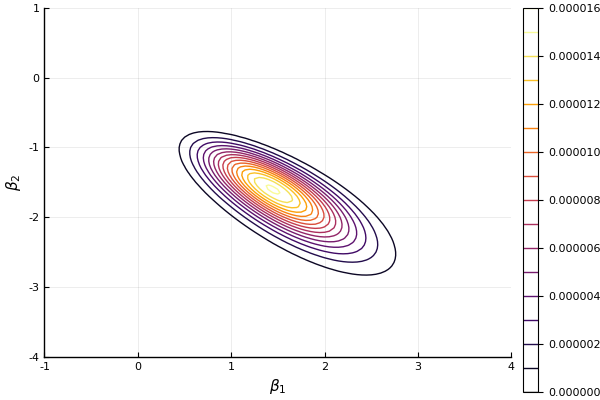
\includegraphics[width=10cm]{images/Ex6_2.png}
    \caption{ Contour plot for 
    $p(\beta \mid Y)$
    }
    \label{fig:2}
\end{figure}

\item Running Metropolis-Hasting algorithm with 10.000 steps.
\begin{figure}[H]
    \centering
    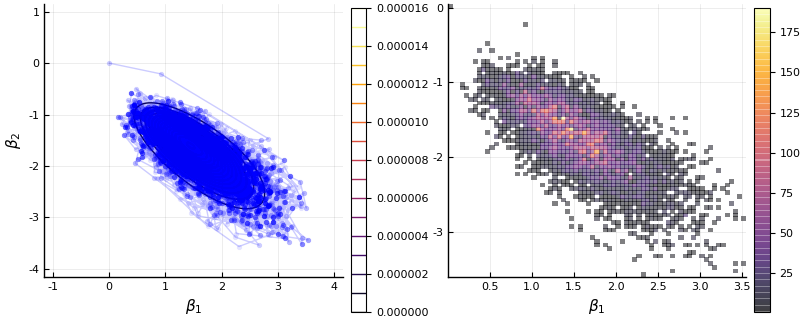
\includegraphics[width=15cm]{images/Ex6_3.png}
    \caption{ Left showing each step of the chain over the distribution.
    Right showing 2D Histogram of the M-H simulation (removing the burnin).
    }
    \label{fig:3}
\end{figure}
\item The trucated normal distributions were implemented to
be used in the Gibbs sampler. Note that $\mathbb I_{Z_i \geq 0}$ has
the same distribution as $Y_i$.

\item Running Gibbs sampler with 10.000 samples.
\begin{figure}[H]
    \centering
    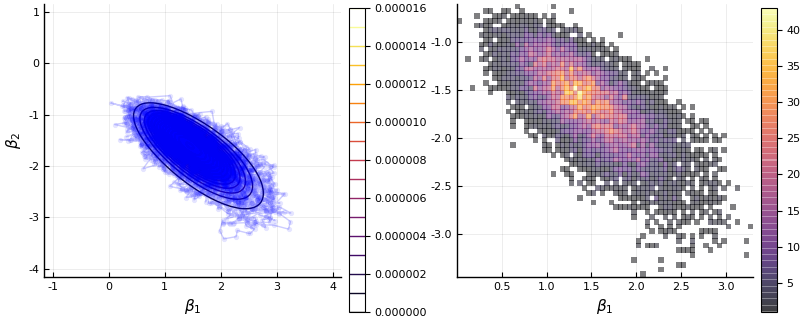
\includegraphics[width=15cm]{images/Ex6_4.png}
    \caption{ Left: Showing each step of the chain over the distribution.
    Right: 2D Histogram of the Gibbs sampler.
    }
    \label{fig:4}
\end{figure}

\item Finally, we compare the performance of each model by evaluating
their autocorrelations.
\begin{figure}[H]
    \centering
    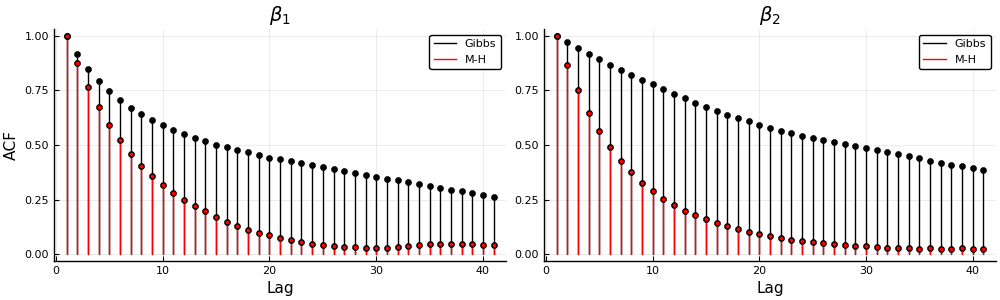
\includegraphics[width=15cm]{images/Ex6_6.png}
    \caption{ Comparison of autocorrelation.
    }
    \label{fig:5}
\end{figure}

\end{enumerate}
\end{document}
